Os pilares são pré-dimensionados para atuarem com uma \textbf{tensão de serviço} ($\sigma$) de $1,0$ a $1,5$ $kN/cm^2$ submetidos a uma ação de $10$ a $12$ $kN/m^2$ por pavimento (carga por pavimento).

Deve-se considerar os seguintes itens para a obtenção das medidas de seção dos pilares:

\begin{itemize}
	\item Espessura dos blocos das paredes adjacentes ($19$ $cm$ para pilares externos e $14$ $cm$ para internos);
	\item Tensão de serviço;
	\item Carga por pavimento;
	\item Número de pavimentos.
\end{itemize}

A carga na base do pilar é o produto: $$F_bi = A_{inf}i \cdot F_{pav} \cdot N_{pav}$$

Onde $F_bi$ é a força na base do pilar $i$ em $kN$, $A_{inf}i$ é a área de influência das lajes adjacentes ao pilar $i$ em $m^2$, $F_{pav}$ é a carga por pavimento em $kN/m^2$ e $N_{pav}$ é o número de pavimentos.

As dimensões da área de influência das lajes em um determinado pilar são montadas a partir da metade da distância até os pilares adjacentes, como na seguinte imagem:

\begin{figure}[h]
	\begin{center}
    	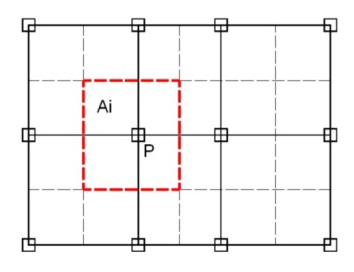
\includegraphics[width=0.5\textwidth]{Pre-dimensionamento-pilares-macicos/Imagens/Area-de-influencia-das-lajes-nos-pilares.jpg}
    	\caption{Área de influência \textit{i} das lajes adjacentes em um pilar \textit{P}.}
	\end{center}
\end{figure}

Obtida a carga na base do pilar, pode-se obter a área da seção pelo quociente, lembrando-se que $\sigma = \lim_{\Delta A \rightarrow 0} \frac{\Delta F}{\Delta A}$, portanto:

$$A_i = \frac{F_bi}{\sigma}$$

Onde $A_i$ é a área da seção transversal do pilar $i$ em $cm^2$, $F_bi$ é a força na base do pilar $i$ em $kN$ e $\sigma$ é a tensão de serviço em $kN/cm^2$.

A \textbf{área mínima} de seção transversal para pilares é de $360$ $cm^2$ e deve ser adotada caso a equação acima dê um valor inferior.

Obtida a área da seção, pode-se finalmente obter a estimativa das dimensões do pilar. Tem-se previamente uma das dimensões (19 $cm$ para pilares externos e 14 $cm$ para internos) e pode-se encontrar a restante a partir da equação da área do retângulo $(base \cdot altura)$ para pilares retangulares.

A nomenclatura das dimensões dos pilares em projetos de estruturas (plantas) é \textbf{Pi (largura x altura)}, por exemplo, \textbf{P5 (19 x 35)}.